\chapter{\ExaHyPE}
\label{section:exahype}


\begin{figure}[htb]
 \begin{center}
  
\includegraphics[width=0.2\textwidth]{60_exahype/EU.png}
  
\includegraphics[width=0.5\textwidth]{60_exahype/ExaHyPE_Logo.jpg}
 \end{center}
 \caption{
   The original ExaHyPE project delivering the first generation of the ExaHyPE
   software has received funding from the European Union’s Horizon 2020 research
   and innovation programme under grant agreement No 671698 (ExaHyPE).
 }
\end{figure}

\noindent
\ExaHyPE\ is the follow-up development of the ExaHyPE project which has been
funded by the EU from 2015--2019.
The present version is the second generation of the code (\ExaHyPE) and has
seen substantial rewrites of core routines.
However, many paradigms and even code blocks remain the same.
Migrating from the original ExaHyPE to \ExaHyPE\ thus should be straightforward.


\ExaHyPE\ is both a set of C/C++ and Fortran core routines complementing the
\Peano\ core and a high-level augmentation of \Peano's Python API.
Compare to the architecture sketch from Chapter \ref{chapter:architecture}.
\ExaHyPE's Python API can be read as builder mechanism:
You configure your particular \ExaHyPE\ application, i.e.~you tell the \ExaHyPE\
engine which application you want to run (which PDE terms, which solver
variants, which hardware properties).
The Python API then yields both a \Peano\ Python project which you can run plus
a set of template classes which you implement with your particular application.


The present document discusses how to create an \ExaHyPE\ application from
scratch.
Most application experts might not want to do this and instead use a read-to-use
\ExaHyPE\ application.
The most prominent (and maybe powerful) code using the ExaHyPE engine is maybe
ExaSeis; used to simulate seismic waves.
The details of these domain-specific codes are not covered by the present
document.



\section*{Preparing \Peano\ to run \ExaHyPE}

It is relatively straightforward to use \ExaHyPE\ within \Peano:

\begin{itemize}
  \item Configure \Peano\ with the flags \texttt{--enable-exahype}
  \texttt{--enable-loadbalancing-toolbox}. These are the two mandatory extensions. You might want to add further options---for VTK and parallelisation, e.g. That is:
  This configuration allows you to run a basic serial \ExaHyPE\ application and
  to write some files in the \Peano\ format, but nothing more.
  \item Recompile your code. This should give you a couple of
  \texttt{ExaHyPE2Core} libraries in the respective subdirectories.
  \item Ensure that \texttt{python} subdirectory is in your Python search path.
\end{itemize}


\section*{Difference of \ExaHyPE\ vs.~ExaHyPE (first generation)}

The original ExaHyPE had been built on top of Peano (third generation) and tried
to hide as much of Peano away as possible.
In \ExaHyPE, I go the opposite way: \ExaHyPE\ is a full-blown Peano add-in and I
try not to hide anything away.
Where we designed our own data management on top of Peano in ExaHyPE, all the
data management (as well as parallelisation, e.g.) is native \Peano.


With the migration from a sole-C++ philosophy to C++ supplemented by a Python
API in \Peano, I also dumped ExaHyPE's former configuration/specification file
pradigma.
An \ExaHyPE\ application now is championed by a sole Python script.
This Python script yields a native \Peano\ application (builder mechanism) which
then assembles the application.



\section{Minimalistic Finite Volumes for the Euler equations}
\label{section:exahype:fv}

I wrote a very simple Finite Volume implementation of a plain Euler solver to
explain the fundamental ideas behind \ExaHyPE.
It is a Jupyter notebook and hosts details explanations.
It also explores different ways how to model the solver, i.e.~I compare
C++-based vs.~symbolic models for all PDE terms.
You can start it via


\begin{code}
cd examples/exahype2/euler
export PYTHONPATH=../../../python
jupyter notebook
\end{code}


\noindent
Alternatively, you can execute the notebook via \texttt{ipython3}.



All calls from the notebook can obviously also be made from a plain Python
script. 
You find examples for such scripts within the subdirectory
\texttt{example-scripts}.


\section{IO and logging}


\ExaHyPE\ codes by default yield snapshots in \Peano's block format. 
That is, there's no distinguished \ExaHyPE\ format.


\paragraph{Explicit VTK conversion with command line tool}
If you have configured \Peano\ with VTK support (\texttt{--with-vtk}), you can
directly convert \ExaHyPE' output files into VTK and visualise these through
Paraview or VisIt.
The command line tool is discussed in Chapter
\ref{chapter:postprocessing}.


There's also a VTK wrapper around the command line tool:

\begin{code}
convert = peano4.visualisation.Convert( "solution-Euler" )
convert.set_visualisation_tools_path( "../../../../src/visualisation" )
convert.extract_fine_grid()
convert.convert_to_vtk()
\end{code}


\paragraph{Direct postprocessing within Paraview}

Paraview offers a Python scripting option. 
Through this scripting interface, you can directly load and manipulate \Peano\
(and hence \ExaHyPE) outputs. 
The interface is also discussed in Chapter
\ref{chapter:postprocessing}.


\paragraph{Logging output}

\ExaHyPE\ searches for a text file \texttt{exahype.log-filter} in the working
directory.
If no such file is found (or the file is corrupted), then it will use some
default filter rules, i.e.~dump the information to the terminal that I consider
to be most important.
If you want to adopt the output, I strongly recommend that you add a log filter
configuration file. 
The syntax of log filter files is discussed in Section
\ref{section:logging:log-filter}.



\section{Running on a parallel computer}

To run \ExaHyPE\ in parallel, you have to build \Peano\ with support for
multithreading and/or MPI.
Once this is done, the engine more or less runs in parallel out of the box.


\paragraph{Domain decomposition}
The core domain decomposition scheme realised in \ExaHyPE\ is a non-overlapping
multiscale domain decomposition based upon space-filling curves (SFC).
To use this scheme, you have to specify an appropriate load balancing scheme.
Without any load balancing, the code will never split up the domain and thus
effectively run serially.

\begin{figure}
 \begin{center}
  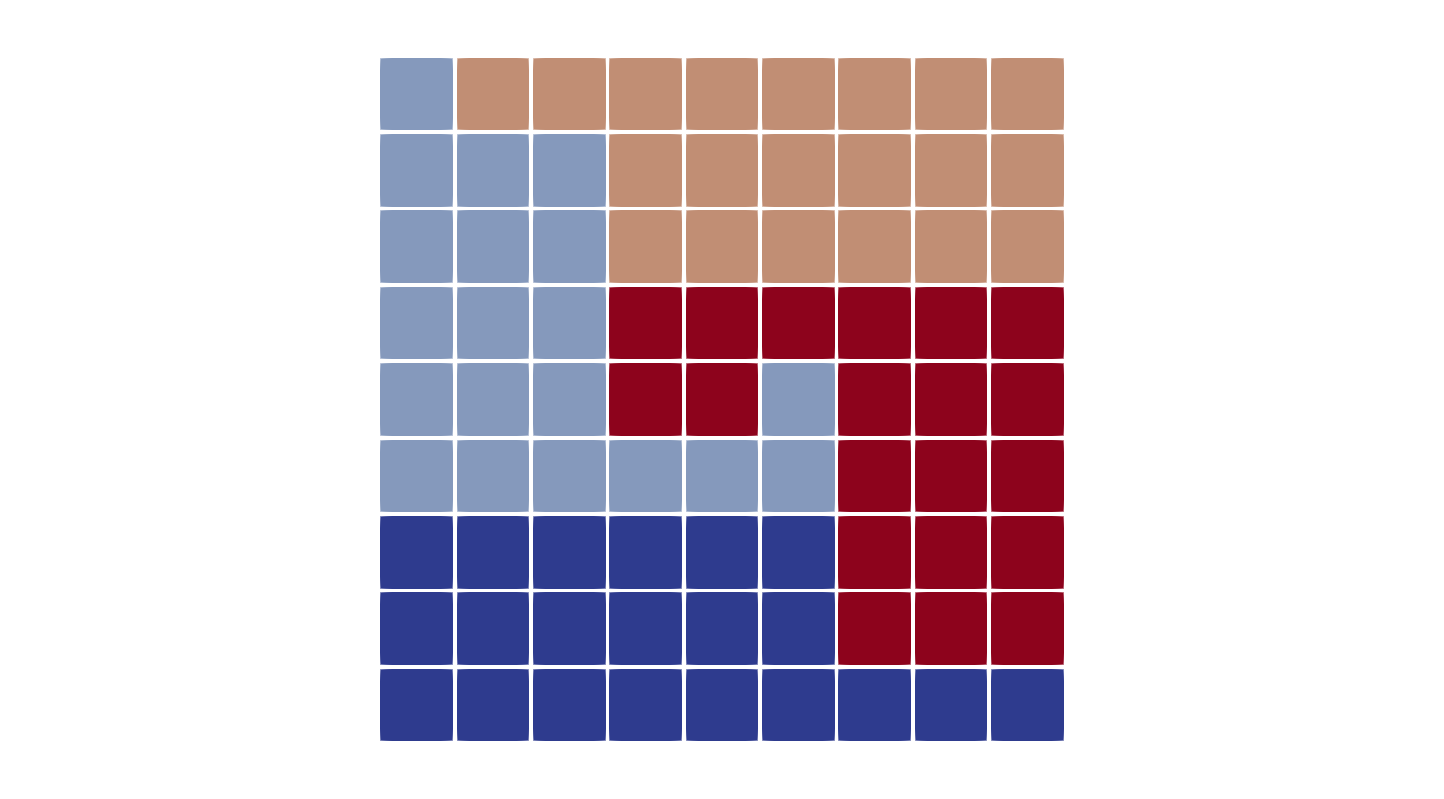
\includegraphics[width=0.54\textwidth]{60_exahype/domain-decomposition.png}
 \end{center}
 \caption{
  Domain decomposition in \ExaHyPE\ for a run with four threads/ranks. Each
  individual cell hosts a patch.
 }
\end{figure}


I plan to support multiple different dynamic load balancing schemes over time,
but the straightforward decomposition scheme shipped with \Peano\ at the moment
is recursive subdivision, a modification of OpenMP's guided scheduling.
To use it, you have to call
\begin{code}
project.set_load_balancing( "toolbox::loadbalancing::RecursiveSubdivision" )
\end{code}

\noindent
on your \ExaHyPE\ project. 


\paragraph{Task parallelism}

Some \ExaHyPE\ solvers add further task parallelism to this decomposition. 
In general, the enclave solvers tend to perform better on massively parallel
systems.


% \paragraph{Task decomposition}
% \ExaHyPE\ realises an additional task decomposition working on top of the domain
% decomposition. 
% This task decomposition is shared memory, only.
% That is, you can use task decomposition without domain decomposition, but then
% you won't benefit from multiple nodes.
% You can however always use domain decomposition without task
% decomposition---though it should be slower in most cases.
% 
% \begin{remark}
% This section is under construction.
% \end{remark} 


\section{GPU support}

To add GPU support (via OpenMP 5), you have to do a couple of steps
and you have to check first whether your solver of choice supports
GPUs. 
Not all solvers are suited for a GPU.
Next, you have to run through a couple of steps:


First, your environment has to be compiled with OpenMP, and I strongly recommend
that you also add \texttt{--with-nvidia} to have support for their tools.
Check that \texttt{-DnoGPUOffloading} is \emph{not} set within the compile
flags and translate your code.
Second, ensure that you use an \ExaHyPE\ solver which has support for GPUs. 
The enclave solvers typically are your solvers of choice.
Solvers that provide GPU support have a flag \texttt{use\_gpu} in their
constructor which is unset by default. 
Set it to \texttt{True} and rerun the toolkit.

\begin{definition}{Solvers with GPU support}
 A solver can use GPUs if and only if can provide all of its PDE terms
 including the eigenvalue computations (so the functions \texttt{flux},
 \texttt{eigenvalues}, \texttt{nonconservativeProducts}, \ldots) as stateless
 functions without side-effects, i.e.~functions that can be written down as
 static and do not need (or even alter) any attribute of the solver class.
\end{definition}

\noindent
If you solver does not fit to this class, it is not a fit for GPUs.
If it fits, then please create two versions of the eigenvalue function and all
of the PDE term functions (such as the flux computations) in your solver.
Keep the original one, and add a second one which is 

\begin{itemize}
  \item static and 
  \item accepts an additional flag of type \texttt{
  tarch::multicore::TargetDevice}.
\end{itemize}

\noindent
You will need to include 
\begin{code}
#include "tarch/multicore/multicore.h"
\end{code} 

\noindent
explicitly. Very often, the standard flux and eigenvalue routines can invoke the
static variants and you can thus eliminate redundancies.
Please note that solvers with GPU support still can have states in their PDE
terms, i.e.~alter solver variables.
But they can do so only for cells which we call skeletons (see the paper by
Charrier et al.~on enclave tasking).


Finally, add
\begin{code}
#if defined(GPUOffloading)
#pragma omp declare target
#endif

my new static function variants

#if defined(GPUOffloading)
#pragma omp end declare target
#endif
\end{code} 






\section{Modelling the fluxes and Riemann solvers with SymPy}

You can model your fluxes, Riemann solvers and so forth with SymPy, 
i.e.~through symbolic formulations---as long as you use a generic numerical
Riemann solver such as Rusanov.
The \ExaHyPE\ SymPy wrapper is
held within the \ExaHyPE\ subpackage \texttt{exahype2.sympy}.


I provide a couple of classes for different PDE variants that should be
compatible to particular \ExaHyPE\ Finite Volume and ADER-DG solvers.
All SymPy classes wrap around SymPy's symbolic expressions, and thus allow users
to work with these expressions directly.
Once you have finished you modelling, the wrappers offer some code generation
which again decorate SymPy's code generation, adds some glue code and can inject
the generate into a \Peano\ solver.


The Euler equations modelled via this interface then add the following code
snippet to the Python script that models \Peano:

\begin{code}
import sympy
import exahype2.solvers.sympy.FirstOrderConservativePDEFormulation


#
# Create a new instance of symbolic ExaHyPE PDE interface.
#
pde = exahype2.solvers.sympy.FirstOrderConservativePDEFormulation(unknowns = 5,dimensions = 3)

#
# Give entries in input vector symbolic names. We first declare some
# helpers/constants. Then we tell the solver how we would like to name the Q 
# entries
#
gamma = sympy.symbols( "gamma")
rho   = pde.name_Q_entry( 0, "rho" )
j     = pde.name_Q_entries( 1, 3, "j" )
E     = pde.name_Q_entry( 4, "E" )

#
# Finally, define the equation system
#
p = (gamma - 1 ) * (E-1/2 * exahype2.solvers.sympy.dot(j,j) / rho)

pde.F[0,:]   = j
pde.F[1:4,:] = 1/rho * exahype2.solvers.sympy.outer(j,j) + p * sympy.eye(3)
pde.F[4,:]   = 1/rho * j * (E+p)

c = sympy.sqrt( gamma * p /rho )
pde.eigenvalue[0] = [ j[0]/rho - c, j[1]/rho - c, j[2]/rho - c ]
pde.eigenvalue[1] = [ j[0]/rho, j[1]/rho, j[2]/rho ]
pde.eigenvalue[2] = [ j[0]/rho, j[1]/rho, j[2]/rho ]
pde.eigenvalue[3] = [ j[0]/rho, j[1]/rho, j[2]/rho ]
pde.eigenvalue[4] = [ j[0]/rho + c, j[1]/rho + c, j[2]/rho + c ]

pde.substitute_expression( gamma, 1.4 )
\end{code}


\noindent
This \texttt{pde} object here can create C++ code that we can plug directly into
the respective \Peano\ routines:
\begin{code}
my_solver.set_implementation( flux=pde.implementation_of_flux(),eigenvalues=...
\end{code}

\noindent
With this call, the modelled PDE feeds, via code generation, directly into the
\ExaHyPE\ solver. When we remodel the PDE, everything is updated automatically.


If you study the interface of \texttt{set\_implementation}, you will notice that
you can also model boundary or initial conditions this way.
In this example, we however only modelled flux and eigenvalues.
The remaining callbacks remain plain C++.


For further resources, please visit SymPy's homepage, and maybe you also want to
have a look into projects like EinsteinPy or galgebra which provide tools for
astrophysics or geometric algebra, respectively.
As we rely on SymPy and expose all the SymPy expressions, they are compatible
with \ExaHyPE.




\section{Finite Volumes with ClawPack (ExaClaw)}

ExaClaw is an add-on to \ExaHyPE\ which makes
the ClawPack Riemann solvers available within \ExaHyPE.
Its development has been made possible by EPSRC under the Excalibur
Phase I call.
The grant number is EP/V00154X/1.



To use this solver family, clone the repository from
\url{https://github.com/clawpack/riemann}.
Furthermore, please ensure that you have configured a Fortran compiler through
\texttt{configure}, i.e.~that you have set the variable \texttt{FC}.
If you have a Fortran compiler in the path by default, everything should work
out-of-the-box.

\begin{remark}
 This solver family is work-in-progress.
\end{remark}



% \section{Ghoddess DG solvers}
% % 
% % We also do provide an interface to Ghoddess DG solvers.
% % Ghoddess solvers use a classic DG formulation with explicit time stepping.
% % Their big USP within \ExaHyPE\ is they rely on a quasi-symbolic formulation and
% % thus facilitate even fast prototyping.
% % 
% \begin{remark}
%   This yet has to be written.
% \end{remark}
 


\section{Introducing a new numerical scheme}

This section discusses how to introduce a totally new numerical solver. 
It does not discuss how to introduce a new PDE, as new PDEs are built on top of
\ExaHyPE.
This section gives you an idea how to extend \ExaHyPE\ instead.

\begin{remark}
  \ExaHyPE\ is a very high level Python API which generates a \Peano\
   Python project which in turn creates the ``real'' \Peano\ C/C++ code. If you
   introduce a new numerical scheme/solver to \ExaHyPE, you thus might want to
   familiarise yourself with \Peano's Python API and how to extend it. This
   recommendation affects all the gluecode/framework aspects of the software.
   All the core numerics of \ExaHyPE\ are held as C++ code in the
   \texttt{src/exahype2} directly and compiled into a separate library. If you
   introduce new numerical schemes, you might have to extend this library, too.
\end{remark}



\subsection{A new Finite Volume solver (native \ExaHyPE)}

Introducing a new Finite Volume scheme is reasonably straightforward within
\ExaHyPE.
It relies directly on \Peano's patch-based AMR.


\begin{itemize}
  \item Create a new subclass of \texttt{exahype2.solver.FV}.
  \item If you class is called \texttt{XYZ}, create four text files:
  \texttt{XYZAbstract.template.h}, \linebreak \texttt{XYZAbstract.template.cpp},
  \texttt{XYZ.template.h} and \texttt{XYZ.template.cpp}. These are Jinja
  templates, and they define your solver (abstract variants) and provide a
  template for routines that a user has to fill in.
\end{itemize}


\paragraph{The C classes/templates}

\ExaHyPE's design concept is that each solver yields two types of classes:
The actual solver and an abstract superclasses. 
Abstract superclasses are regenerated every time you rerun the Python script.
Furthermore, they define the whole signature, i.e.~if you alter the signature
later on, users simply rerun the toolkit. 
Finally, the abstract superclasses hold default implementations\footnote{Some
solvers do not expect the user to write any C/Fortran code at all. In this
case, the solvers nevertheless should create an abstract superclass (now
holding all functions) and a subclass which is basically empty. This way, we
are consistent.}.


With \Peano, you can create arbitrary abstract superclasses. 
They have to implement \texttt{exahype2::Solver} though.


\paragraph{The Python code}


The core implementation effort clearly has to go into the parts where the actual
mesh traversal is mapped onto solver calls.
In \ExaHyPE, this is realised through templates. 
Any Finite Volume code relies basically on four templates:

\begin{itemize}
  \item \texttt{AMRTemplate} will be called on solver cells to determine whether
  to refine or erase.
  \item \texttt{AdjustCellTemplate} will be called to impose initial conditions
  or interior ones.
  \item \texttt{HandleBoundaryTemplate} is invoked for boundary faces.
  \item \texttt{HandleCellTemplate} is the actual Finite Volumes solver
  invocation.
\end{itemize}


\noindent
These four strings are Jinja templates. The idea is that particular FV
subclasses ``overwrite'' (set) them and thus inject their solver behaviour.
Each handle is guarded by an additional expression (some C++ code evaluating to
boolean) to switch it on/off.
There's two more things that are automatically done: patch updates are
automatically projected onto the faces, and the projected face data is
automatically rolled over.
While these things are ``hard-coded'', you still have guards to switch it
on/off.


The template mechanism works similar to aspect-oriented programming, i.e.~it
simply enables Python to plug some code snippets straight into your the
generated \ExaHyPE\ code. 
For a list of predefined constants that are available within the templates,
please consult the routine
\texttt{\_init\_dictionary\_with\_default\_parameters} which befills a lookup
table.
You can, obviously, add more entries within your implementation.
For this, a solver has to implement
\texttt{add\_entries\_to\_text\_replacement\_dictionary}.
Some of the most important preset dictionary entries are:


\begin{itemize}
  \item \texttt{fineGridCell\{UNKNOWN\_IDENTIFIER\}.value} which is a double
    pointer which points to the whole patch hosted by the cell in the volumetric
    routines \texttt{CreateCellTemplate}, \texttt{HandleCellTemplate} and
    \texttt{AMRTemplate}. The array it points to has the size \linebreak
    \texttt{\{NUMBER\_OF\_VOLUMES\_PER\_AXIS\}}$^d \cdot $
    \texttt{\{NUMBER\_OF\_UNKNOWNS\}}.
  \item \texttt{fineGridFace\{UNKNOWN\_IDENTIFIER\}.value} is the face
    equivalent for the boundary conditions. Again, it is a double pointer,
    though one dimension is not equal to
    \texttt{\{NUMBER\_OF\_VOLUMES\_PER\_AXIS\}} but equal to the halo overlap.
    See the Finite Volumes discussion in
    Chapter~\ref{section:python-api-examples:finite-volumes}.
  \item \texttt{reconstructedPatch} and \texttt{originalPatch} are only defined
    within \texttt{HandleCellTemplate}. The former is an alias for
    \texttt{fineGridFace\{UNKNOWN\_IDENTIFIER\}.value}, i.e.~points to the same
    location. \texttt{reconstructedPatch} is another pointer which points to the
    patch from the previous mesh traversal, i.e.~you can overwrite data
    within \texttt{originalPatch} and still have the old one available.
    Furthermore, the underlying patch is bigger: It hosts the actual patch data
    plus its halo.
\end{itemize}




\begin{remark}
 If you want to see a really simple example of this solver type, change into the 
 directory \texttt{src/exahype2/fv} and have a look into \texttt{Rusanov.cpp}.
 It follows exactly the above recipe.
\end{remark}


\noindent
I see two different paradigms how to realise a new solver: 
You can either code your solver directly within the Python templates.
Alternatively, you can generate some generic glue code within the template and
forward calls to some C++ which can either stem from a library or be user
code.


Both variants have pros and cons and are valid.
For my generic Rusanov solver (as well as for ADER-DG), we can realise all
numerics generically within predefined kernels relying only on few user-defined
functions injecting flux and eigenvalues.
Furthermore, these functions have the same signature for all applications.
For a bespoke Finite Volume scheme where the Riemann solver holds the actual
numerical wisdom and each Riemann solvers requires a bespoke signature, it is
maybe better to skip that additional level of abstraction.



% \subsection{Ghoddess implementation remarks}
% 
% Ghoddess works on triangles which we embed into the squares or cubes,
% respectively, of \ExaHyPE.
% By default, the code employs Gauss-Legendre sample points.
% The data structure used thus read as follows
% (Fig.~\ref{figure:60_exahype:degree-of-freedom-layout:Ghoddess}):
% \begin{itemize}
%   \item The solver embeds a ``patch'' of $N$ polynomial weights into each cell.
%   For order $p=1, d=2$, we have for example $N=6$, for $p=2, d=2$ we have
%   $N=12$.
%   \item Each face carries $2(p+1)^{d-1}$ doubles.
% \end{itemize}
% 
% 
% \noindent
% The face data holds a left and a right representation of the polynomial along
% the face.
% So it does not really hold degrees of freedom.
% Its degree of freedom are mere projections of the cell solution onto the face.
% 
% 
% 
% \begin{figure}
%  \begin{center}
%   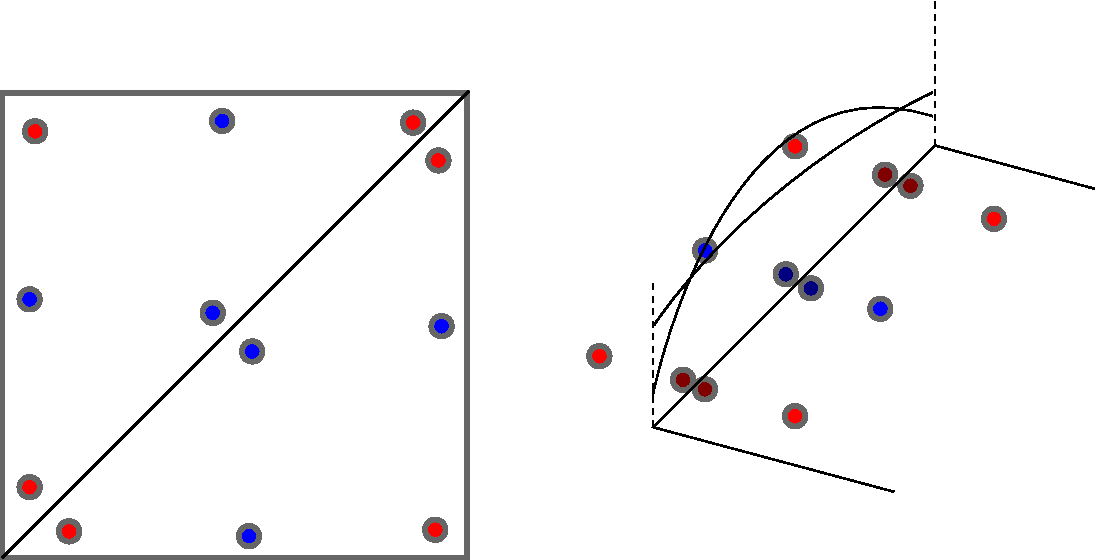
\includegraphics[width=0.65\textwidth]{60_exahype/Ghoddess-dof-layout.pdf}
%  \end{center}
%  \caption{
%   Left: Degree of freedom layout in Ghoddess within a cell.
%   Right: Each face holds additional ``degree of freedoms'' which encode the
%   projection of the cell polynomial onto the face.
%   \label{figure:60_exahype:degree-of-freedom-layout:Ghoddess}
%  }
% \end{figure}
% 
% The Ghoddess solver itself splits up into four computation kernels:
% 
% \begin{enumerate}
%   \item The {\bf projectOntoFace} kernel accepts the $N$ degrees of freedom from
%   the cell and projects the polynomials of the two triangles within the cell
%   onto the faces. It consequently writes $2d \cdot (p+1)^{d-1}$ face DoFs. Once
%   we have traversed the whole mesh, each face ``knows'' its left and right
%   projection.
%   \item The {\bf solveRiemann} kernel takes the $2 \cdot (p+1)^{d-1}$ DoFs on
%   the face, i.e.~the left and right projection, and solves the Riemann problem
%   on the jump. The result is written back into the $2 \cdot (p+1)^{d-1}$ DoFs.
%   In principle, this allows us to have a different outgoing flux for the left
%   and right side of a face.
%   \item The {\bf solveCell} kernel evolves the solution within the triangle
%   pair, i.e.~it evaluates the volumetric integrals of the DG formulation. The
%   name is slightly wrong: Besides the volumetric terms, the kernel also
%   evaluates the face terms arising between the two triangles embedded into the
%   cell. So it is a combination of a cell kernel plus one Riemann solve (in 2d).
%   \item The {\bf projectOntoCell} kernel takes the Riemann solution on the cell
%   faces, i.e.~the output of projectOntoFace, and adds it to the cell solution,
%   i.e.~it adds it to the outcome of solveCell.
% \end{enumerate}
% 
% 
% \noindent
% Ghoddess' vanilla version indeed traverses the mesh four times per time step.
% This makes it easy/easier to debug the code and to analyse the substeps.
% The work of Charrier et al then automatically fuses the traversals and thus
% reduces the memory accesses and homogenises the computational character over the
% mesh sweeps.
% 
% 
% The realisation of the four sweeps relies on blockstructured extension of
% \Peano:
% Though the data is logically not Cartesian or block-structured, we model all
% properties as blocks embedded into the mesh.
% 
% 
% All solvers inherit from \texttt{exahype2.ghoddess.Solver} which is our abstract
% framework.
% Per solver, the Python API will generate one C++ solver class.
% This class has a couple of things to do:
% 
% \begin{enumerate}
%   \item It holds all time stepping data. So it knows, for example, what the
%   minimal time stamp at the moment is.
%   \item It serves as a state machine which decides at any point which kernels
%   are to be executed on particular grid entities.
%   \item It holds the application domain-specific routines such as the actual
%   kernel implementations, refinement criteria or data initialisation.
% \end{enumerate}



\section*{Links and further reading}

\begin{itemize}
  \item The ``official'' ExaHyPE release paper is
{\tiny \begin{verbatim}
@article{Reinarz:2019:ExaHyPE,   
  title = "ExaHyPE: An engine for parallel dynamically adaptive simulations of wave problems",
  journal = "Computer Physics Communications",
  pages = "107251",
  year = "2020",
  issn = "0010-4655",
  doi = "https://doi.org/10.1016/j.cpc.2020.107251",
  url = "http://www.sciencedirect.com/science/article/pii/S001046552030076X",
  author = "Anne Reinarz and Dominic E. Charrier and Michael Bader and Luke Bovard and Michael Dumbser 
    and Kenneth Duru and Francesco Fambri and Alice-Agnes Gabriel and Jean-Matthieu Gallard and 
    Sven Köppel and Lukas Krenz and Leonhard Rannabauer and Luciano Rezzolla and Philipp Samfass and 
    Maurizio Tavelli and Tobias Weinzierl",
  keywords = "Hyperbolic, PDE, ADER-DG, Finite volumes, AMR, MPI, TBB, MPI+X",
}
  \end{verbatim}}
  If you use the software, it would be great if you could cite this one.
\end{itemize}

